
%(BEGIN_QUESTION)
% Copyright 2006, Tony R. Kuphaldt, released under the Creative Commons Attribution License (v 1.0)
% This means you may do almost anything with this work of mine, so long as you give me proper credit

A water control valve is supposed to pass a maximum flow rate of 300 GPM from the pump to the storage vessel, to hold the vessel's level constant at the setpoint shown:

$$\includegraphics[width=15.5cm]{i01408x01.eps}$$

The pump's outlet pressure is a constant 50 PSI, and we will assume the vessel's level remains constant at 10 feet.  Given these conditions, calculate the flow capacity ($C_{v}$ rating) for this control valve.  Also, determine whether or not there is enough information given in this P\&ID to indicate the control valve's action (either signal-to-open or signal-to-close).

\vskip 20pt \vbox{\hrule \hbox{\strut \vrule{} {\bf Suggestions for Socratic discussion} \vrule} \hrule}

\begin{itemize}
\item{} Explain how you may use the known height of water in the vessel to calculate the valve's downstream pressure ($P_2$).  There is more than one way to do this!
\item{} What do the symbols and line types tell you about the individual instruments used in this level control system?
\item{} Suppose operations personnel decided to raise the setpoint in this level control system from 10 feet to 15 feet.  Would this operational change affect the required control valve size (assuming we still need 300 GPM maximum flow)?  Why or why not?
\item{} Suppose electricians installed a {\it VFD} (``variable-frequency drive'') in the pump motor electrical system, allowing the AC induction motor to be run at less than 100\% speed to conserve energy.  Would a reduced pump speed affect the required control valve size (assuming we still need 300 GPM maximum flow)?  Why or why not? 
\item{} Suppose the sliding-gate valve on the discharge line from this liquid storage vessel were replaced with one having a smaller pipe size.  Would this hardware change affect the required control valve size (assuming we still need 300 GPM maximum flow)?  Why or why not?
\end{itemize}

\underbar{file i01408}
%(END_QUESTION)





%(BEGIN_ANSWER)

$C_{v}$ = 44.395

%(END_ANSWER)





%(BEGIN_NOTES)

Ignoring frictional losses in the pipe (i.e. downstream valve pressure is stricly a function of hydrostatic head):

$$\Delta P = 50 - \left(10 \hbox{ ft WC} \over 1 \right)  \left(12 \hbox{ in} \over 1 \hbox{ ft}\right)  \left(1 \hbox{ PSI} \over 27.68 \hbox{ "WC}\right) = 45.66 \hbox{ PSID}$$

$$Q = C_v \sqrt{\Delta P \over G_f}$$

$$C_v = {Q \over \sqrt{\Delta P \over G_f}}$$

$$C_v = {300 \over \sqrt{45.66 \over 1}} = 44.395$$



\vskip 10pt

A very important detail in this question is the word ``maximum.''  It is important to know that 300 GPM is the maximum flow rate, because otherwise we may risk undersizing the valve.  A valve with a (100\% wide-open) $C_v$ of 44.395 will yield a water flow of 300 GPM at the specified pressure and controlled height, {\it but no more}.  If 300 GPM were the {\it normal} flow rate and not the {\it maximum} flow rate, we would need a control valve with a larger (wide-open) $C_v$.

\vskip 10pt

It should be noted that the control valve's action is un-described by this P\&ID.  We have no idea, just by examining the diagram, which way this control valve actuates.  One {\it cannot} infer the valve's action from the placement of the air line on the diaphragm actuator.  Some students see how the air line connects, and assume this means air-to-close, but often times such symbols (especially in a PFD or P\&ID) are generic and do not necessarily imply which side of the diaphragm the air line goes.

\vskip 20pt \vbox{\hrule \hbox{\strut \vrule{} {\bf Virtual Troubleshooting} \vrule} \hrule}

This question is a good candidate for a ``Virtual Troubleshooting'' exercise.  Presenting the diagram to students, you first imagine in your own mind a particular fault in the system.  Then, you present one or more symptoms of that fault (something noticeable by an operator or other user of the system).  Students then propose various diagnostic tests to perform on this system to identify the nature and location of the fault, as though they were technicians trying to troubleshoot the problem.  Your job is to tell them what the result(s) would be for each of the proposed diagnostic tests, documenting those results where all the students can see.

During and after the exercise, it is good to ask students follow-up questions such as:

\begin{itemize}
\item{} What does the result of the last diagnostic test tell you about the fault?
\item{} Suppose the results of the last diagnostic test were different.  What then would that result tell you about the fault?
\item{} Is the last diagnostic test the best one we could do?
\item{} What would be the ideal order of tests, to diagnose the problem in as few steps as possible?
\end{itemize}

%INDEX% Final Control Elements, valve: sizing

%(END_NOTES)


